\documentclass[12pt]{article}

\usepackage{hyperref} %links in ToC
\usepackage{caption} %interesting things with captions
\usepackage[margin=1.5in]{geometry} %mostly set margin of the report
\usepackage{tabulary} %text wrapping in tables
\usepackage{subcaption} %let me put multiple images into a single caption
\usepackage{textcomp} %let me use \textrangle{} to get '>'

%images being embeded
\usepackage{graphicx}
\graphicspath{ {images/} }

%code highlighting
\usepackage{minted}
\setminted[c++]{frame=single,linenos=true,autogobble=true,numbersep=4pt,tabsize=4}
\setminted[bash]{frame=single,linenos=true,autogobble=true,numbersep=4pt,tabsize=4}
\setminted[xml]{frame=single,linenos=true,autogobble=true,numbersep=4pt,tabsize=4}

%fix a quote mark issue
\usepackage [english]{babel}
\usepackage [autostyle, english = american]{csquotes}
\MakeOuterQuote{"}


\begin{document}
\pagenumbering{gobble}
\begin{titlepage}
	\centering
	{\Huge Virtualisation\par}
	\vspace{0.25in}
	{\Large Project 1\par}
	\vspace{2in}
	{Alex Harper\par}
	\newpage
\end{titlepage}
\pagenumbering{roman}
\tableofcontents
\newpage

\listoffigures
% \listoftables
\newpage
\setlength{\parindent}{4em} %indent of first line of paragraph
\setlength{\parskip}{1em} %space between paragraphs

\pagenumbering{arabic}

% \section{topics}
% \begin{verbatim}

% ---ADDING TESTS TO GLOP CONFIG---
% if i need to pad more pages, but i want to try not haing to do this
% \end{verbatim}

\section{Introduction}

This project has been my first time using Visual Studio and git on Windows.
While I do not really like either things, they do work if you use them correctly.
In this paper I go over what I did to get ready for working with Windows for programming as well as some specific programming bits.

The programming I show here is mostly for me to play with Visual Studio to work out what quirks it has.
I took that opportunity to get Goole Test setup in a project and do some basic tests, which was a bit of a learning curve for me.
For the tests, I was pushing how far I could get bad code to still work correctly by doing obviously wrong things.
I also give some basic code examples of making classes, because that is what the book goes over.

\section{Visual Studio}

Since I am always the odd man out by using linux, I have to cave and meet the enviroment that my group partners are going to be using.
This means Windows and Visual Studio.
I have touched Visual Studio before in the form of the reskined Atmel Studio to do micro controller programming, but that was fairly different than the original.

Installing the IDE was simple with downloading the installer and running it.
It gave some options and I made sure to get the C++ compiler installed.

\begin{figure}[ht]
	\centering
	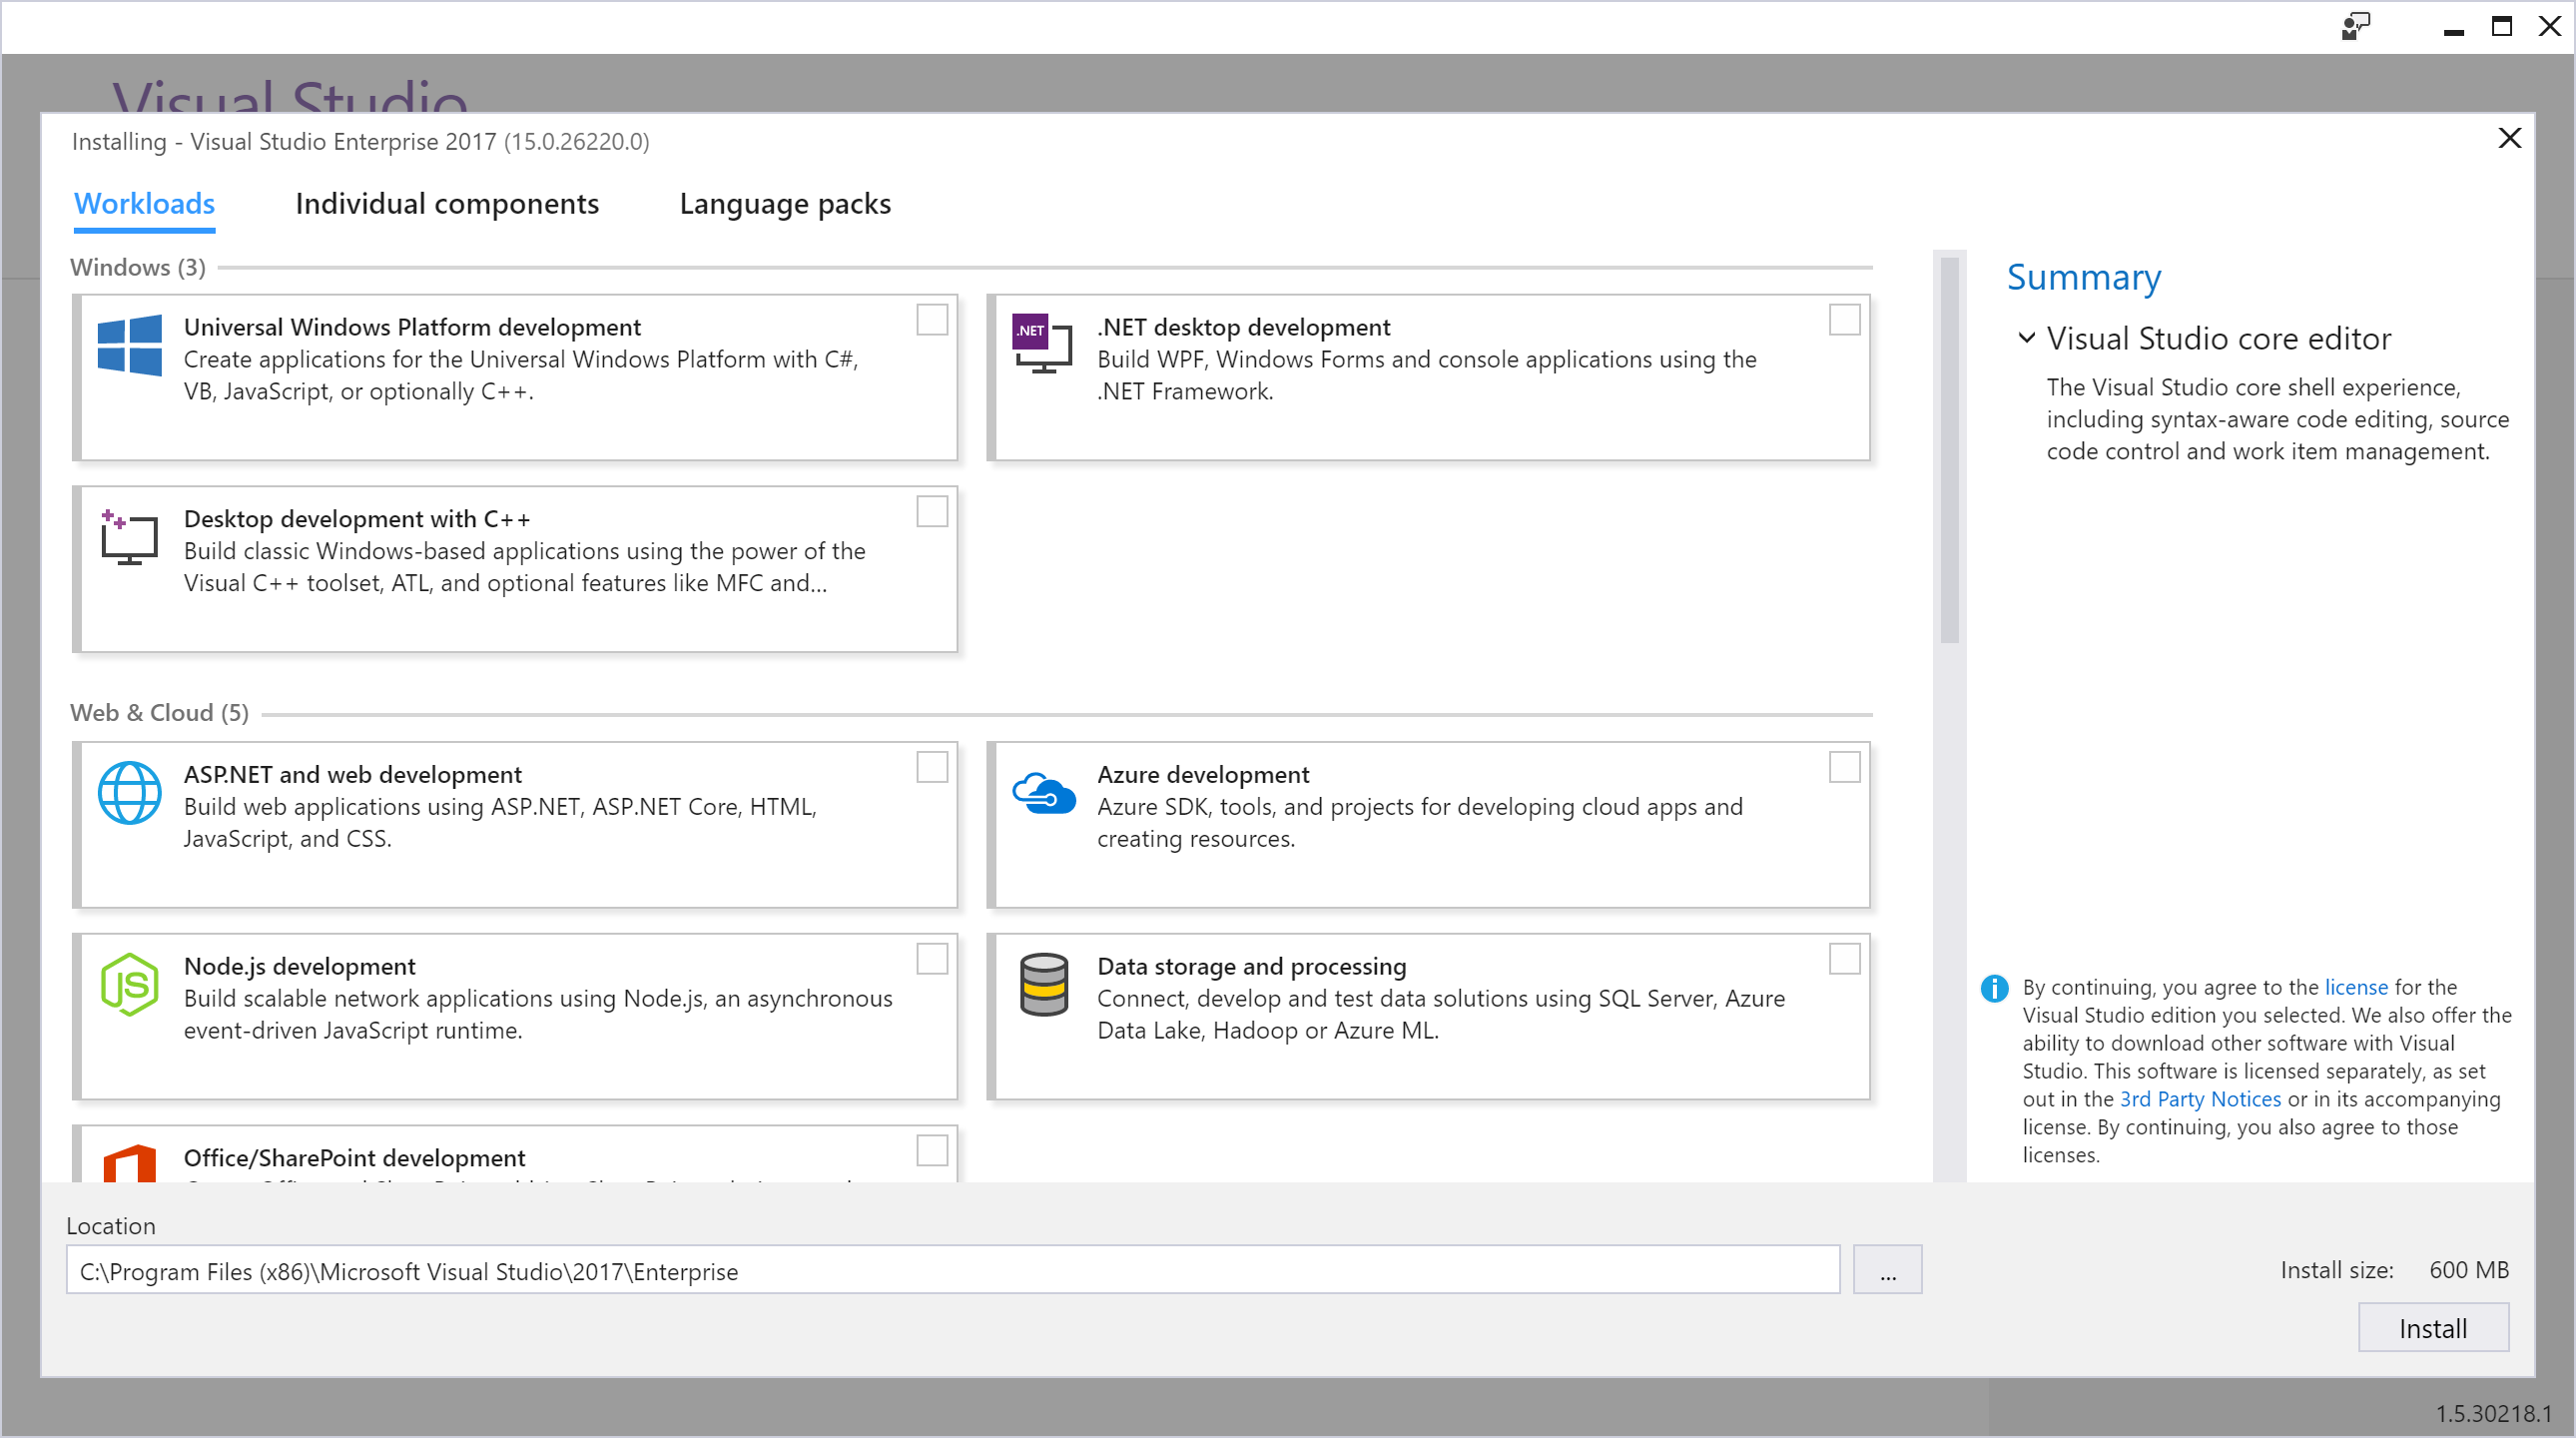
\includegraphics[width=\textwidth]{vs_installer.png}
	\caption{Window of Installer to Select extra Components}
	\label{fig:vs_installer}
\end{figure}

After getting installed, it was time to mess around with it and see what it is like.
I made a new "solution" and made sure the compiler worked, and that things operated for the basics.
It is fairly similar to what I have used before, just different keyboard bindings.

After messing around a few minutes, I made a list of things I don't like about the program, but in general are not very major.
\begin{itemize}
	\item Missing Features that I am used to having
	\begin{itemize}
		\item When the variable is a pointer to an object, pressing the '.' button does not automatically translate it into '-$>$'
		\item The suggestions pane while typing does not automaticly come back when I accidentally dismiss it (but ctrl+space brings it up)
		\item The suggestions pane while typing does not select the first entry in the box  by default and waits for me to press the down button. This messes me up a lot with my muscle memory
		\item The block comment shortcuts are stupid. It should be a toggle of commenting the block and not make the person have to remember two different buttons.
		\item The "toggle header/source file" shortcuts don't even work
	\end{itemize}
	\item When asking it to build or start a test, it takes a second or two to even start the process. There is no reason it should take that long
	\item It broke on me once, simply not building. A simple restart of the program fixed it, but why did it decide to stop working?
	\item There seems to be no way to select a location in a repository to put a solution made in visual studio, making me have to externally manage it. Not a huge deal
\end{itemize}

\section{Google Test}

For the testing framework, our group has decided to use Google Test.
It is a simple framework that lets you simply define a group of code and explicitly set test conditions.
The framework handles running the tests and trys to gracefully handle any exceptions in the tests (and marks those as failures).
To install the framework, it was simple with the built in tool that manages extra plugin stuff for Visual Studio.
In the start menu search for "visual studio installer" and then click the buttons shown in fig\ref{fig:modify_button} and fig\ref{fig:google_test_plugin}.

\begin{figure}[ht]
	\centering
	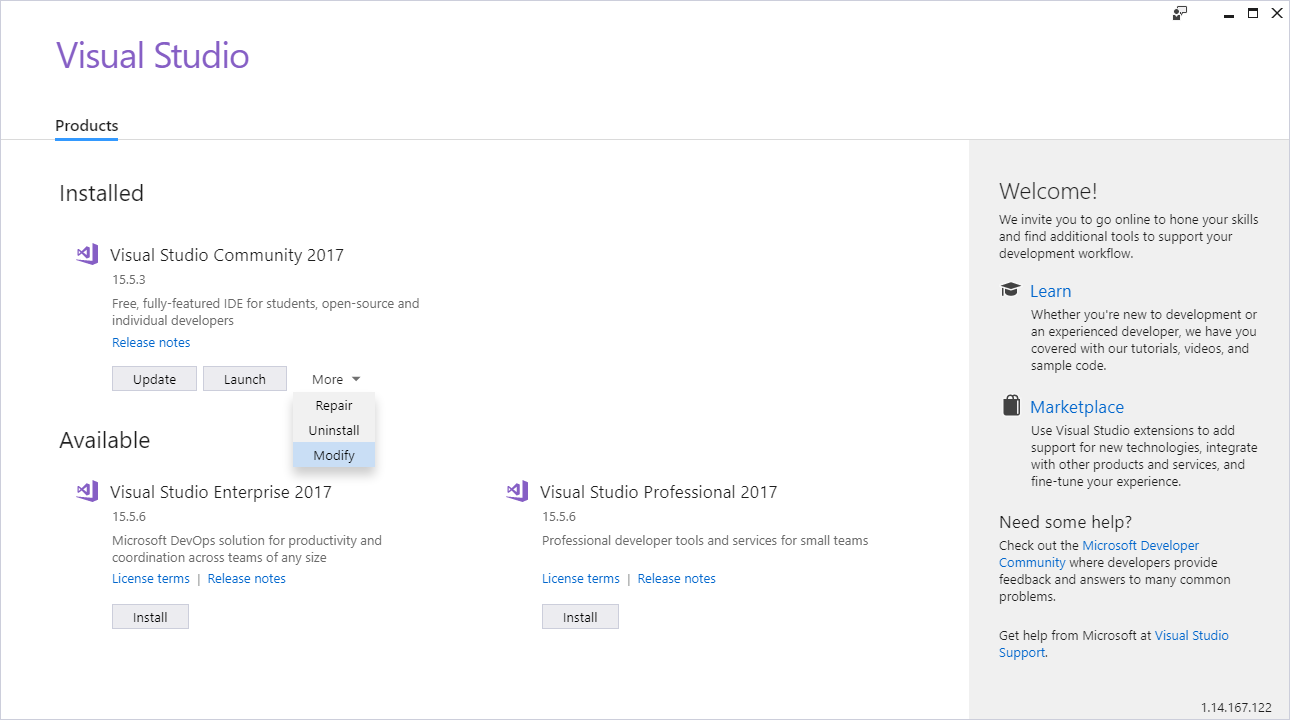
\includegraphics[width=\textwidth]{modify_button.png}
	\caption{Button To Press In The "Installer" To Add Components To Visual Studio}
	\label{fig:modify_button}
\end{figure}

\begin{figure}[ht]
	\centering
	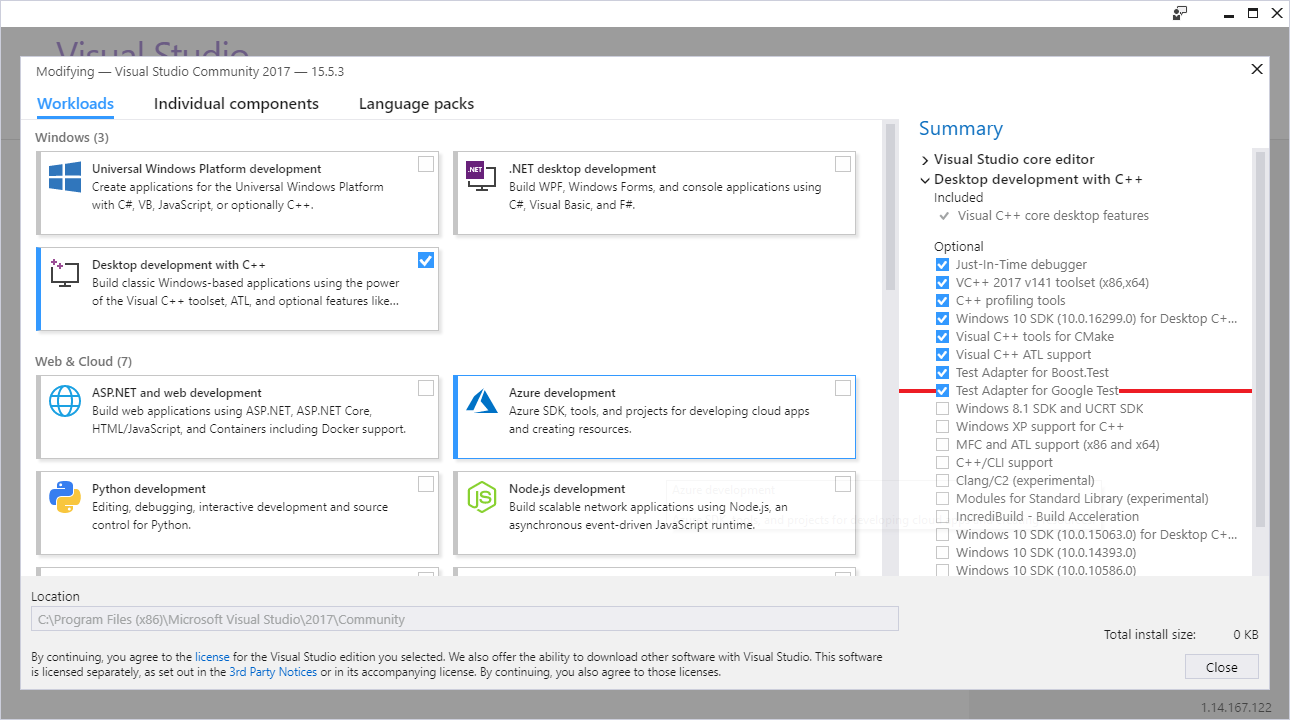
\includegraphics[width=\textwidth]{google_test_plugin.png}
	\caption{Checkbox Location For Google Test - Highlighted In Red}
	\label{fig:google_test_plugin}
\end{figure}

After getting it installed, it is time to make a new project to use google test.
This is where I got confused and spen about an hour going in circles.
Visual Studio has two different things of a "solution" and a "project".
Only a single solution can be open at a time, but it can contain several projects.
I had thought that they were the same thing and as I went to make a new project, instead I made a new solution.
When you go to "File - New - Project" it defaults to making a new solution at the same time and not putting it in the current solution which already had my code in it.
There is a dropbox for making it add to the current solution, but instead I will continue to opt for what is fig\ref{fig:vs_new_project}.

\begin{figure}[ht]
	\centering
	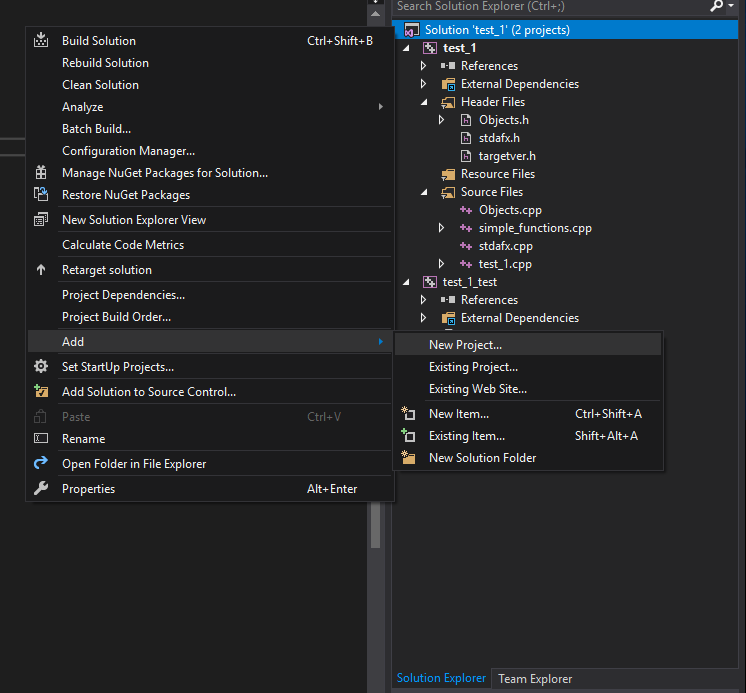
\includegraphics[width=0.6\textwidth]{vs_new_project.png}
	\caption{How I Will Add Projects To My Current Solution From Now On}
	\label{fig:vs_new_project}
\end{figure}

And now that the framework is installed, lets make some tests.
At first I decided to only do super basics, but it devolved into a short exploration of abusing the memory layout of objects and see what technically works and didn't break things.
In fig\ref{fig:example_test} is an example test case that shows the very basic usage.
In fig\ref{fig:test_explorer} shows the test explorer pane in visual studio.

\begin{figure}[ht]
	\centering
	\begin{minted}{c++}
		TEST(TestGroupName, TestName) {
			EXPECT_EQ(1, 1);
			EXPECT_TRUE(true);
		}
	\end{minted}
	\vspace{-15pt}
	\caption{Example Test Case Using Google Test}
	\label{fig:example_test}
\end{figure}

\begin{figure}[!ht]
	\centering
	\begin{subfigure}[t]{0.45\textwidth}
		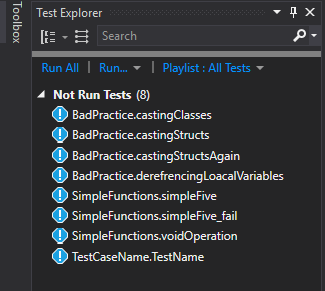
\includegraphics[width=\textwidth]{not_run_tests.png}
		\caption{Tests Before Running Them}
	\end{subfigure}
	\begin{subfigure}[t]{0.45\textwidth}
		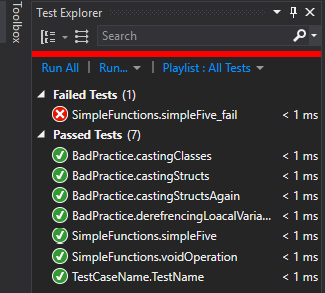
\includegraphics[width=\textwidth]{run_tests.png}
		\caption{Tests After Running Them}
	\end{subfigure}
	\begin{subfigure}[t]{0.45\textwidth}
		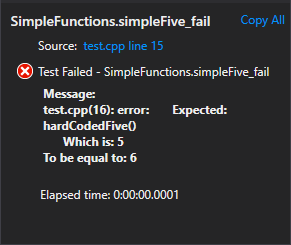
\includegraphics[width=\textwidth]{failed_test_summary.png}
		\caption{Summary of a Failed Test}
	\end{subfigure}
	\caption{Test Explorer Pane In Visual Studio}
	\label{fig:test_explorer}
\end{figure}

\clearpage
\section{Git on Windows}

This is where things took a large departure from what I was expecting.
I am very familure using git with a command line and I like the simplicity of it.
The extension in visual studio is something that I am not used to, as it feels opaque to me.
Really the operation of it is simple and the same as normal git, but I still like my command line.
In fig\ref{fig:team_explorer} is a picture of what the add-on looks like.

\begin{figure}[!ht]
	\centering
	\begin{subfigure}[t]{0.45\textwidth}
		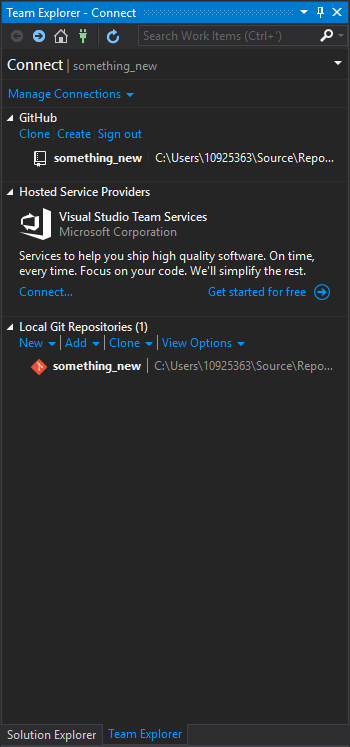
\includegraphics[width=\textwidth]{team_explorer.png}
		\caption{Team Explorer With Github}
	\end{subfigure}
	\begin{subfigure}[t]{0.45\textwidth}
		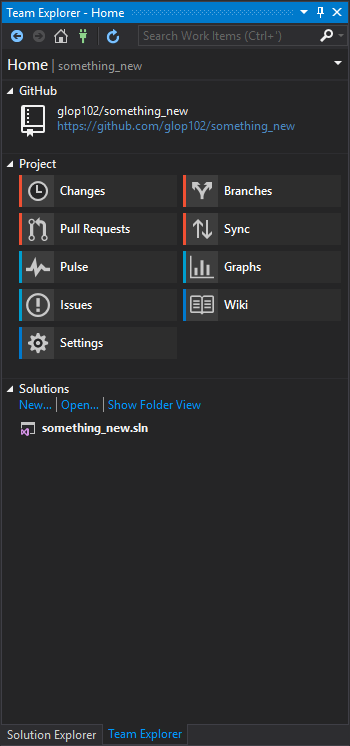
\includegraphics[width=\textwidth]{github_repo.png}
		\caption{Local Repo with Various Buttons}
		\label{fig:repo_buttons}
	\end{subfigure}
	\caption{Team Explorer Pane In Visual Studio}
	\label{fig:team_explorer}
\end{figure}

The team explorer pane is a builtin part of the program already, but is limited to only working with microsoft services.
The github extension adds the extra field of letting github be the back end that code is stored on.
As you can see in fig\ref{fig:repo_buttons}, it has quick access buttons for the typical actions.
The "changes" button is where you make commits to the current branch.
The "sync" button is where you push or pull code.
The "branches" button is where you do merges and such.

After messing with it, I suggest starting by making the new repo with github first.
Place the repo where you want before making the new "solution" in VS.
When you make the new "solution", change the location to the repo folder that was just made.
Now when you go to the changes button with the plugin, it will let you add a commit message and push the files up.
Note: When you make the repo, make sure to have a .gitignore file get made to keep all the trash that visual studio puts in from making your repo get huge in size.

While this seems kindof handy, I still prefer using the command line directly.
I am used to a workflow on the command line under linux.
The idea of an IDE is neat, but I typically only use it for a handy text editor that gives suggestions as I type.
It will be an interesting experiance as I work with my team on this.

\section{Playing With Classes}

As the section fo the book is about how to make classes with various restrictions and features, I suppose I should mention some things about that myself.
I simply added this code into my test project for Google Test.

The book has many pages about specifics of what to do for exact situations.
I instead am just going to give a short list of things here that sumarize the important bits.

\newpage
In fig\ref{fig:class_ex1} is the most simple example subclass you can do in c++.
The test on the right passes.
The first two conditional checks show that things make sense with each returning their own proper names.
The last conditional check has the subclass casted as a base class, and so it returns the name of the base class.

\begin{figure}[!ht]
	\centering
	\begin{tabular}{c c}
		\begin{minipage}[t]{0.45\textwidth}
		\begin{minted}{c++}
			class Base1 {
			public:
				string name();
			};
			class Sub1:public Base1 {
			public:
				string name();
			};
		\end{minted}
		\end{minipage}
		&
		\begin{minipage}[t]{0.5\textwidth}
		\begin{minted}{c++}
			TEST(ClassTest,t1){
				Base1 *a, *bb;
				Sub1 *b;
				a = new Base1;
				b = new Sub1;

				string name = a->name();
				EXPECT_EQ(name, "Base1");

				name = b->name();
				EXPECT_EQ(name, "Sub1");

				bb = (Base1*)b;
				name = bb->name();
				EXPECT_EQ(name, "Base1");

				delete a;
				delete b;
			}
		\end{minted}
		\end{minipage}
		\\
	\end{tabular}
	\caption{Simple Subclass}
	\label{fig:class_ex1}
\end{figure}

\newpage
In fig\ref{fig:class_ex2} is trying to change the last test case.
The way to do this is to declare the name() method as virtual in the base to allow sub classes to override it.
As before, the first two conditional checks have them returning their own proper names.
The last conditional check has the subclass casted as a base class, but this time it still returns the name of the subclass.
This shows how virtual functions can allow extensions to an object without changing code that uses the objects.

\begin{figure}[!ht]
	\centering
	\begin{tabular}{c c}
		\begin{minipage}[t]{0.45\textwidth}
		\begin{minted}{c++}
			class Base2 {
			public:
				virtual string name();
			};
			class Sub2 :public Base2 {
			public:
				string name();
			};
		\end{minted}
		\end{minipage}
		&
		\begin{minipage}[t]{0.5\textwidth}
		\begin{minted}{c++}
			TEST(ClassTest, t2) {
				Base2 *a, *bb;
				Sub2 *b;
				a = new Base2;
				b = new Sub2;

				string name = a->name();
				EXPECT_EQ(name, "Base2");

				name = b->name();
				EXPECT_EQ(name, "Sub2");

				bb = (Base2*)b;
				name = bb->name();
				EXPECT_EQ(name, "Sub2");

				delete a;
				delete b;
			}
		\end{minted}
		\end{minipage}
		\\
	\end{tabular}
	\caption{Virtual Methods for Subclasses}
	\label{fig:class_ex2}
\end{figure}

\newpage
In fig\ref{fig:class_ex3} shows the last major topic in objects.
A static variable is tangentially related to global variables, in that there is only one that everyone shares.
When you declare a thing static in an object, it is going to be the single thing used for all objects of that type.
Say you have a static int and you make 100 objects, all 100 objects would use the exact same int, and not their own copies of it.
Same idea with inheriting a static method, it will be the only method that everyone uses with not even a chance to override it.
That is why in this example the "Sub3" class does not even make it's own.
It is forced to use the base class and not allowed to overwrite it.

\begin{figure}[!ht]
	\centering
	\begin{tabular}{c c}
		\begin{minipage}[t]{0.45\textwidth}
		\begin{minted}{c++}
			class Base3 {
			public:
				static string name();
			};
			class Sub3 :public Base3 {};
		\end{minted}
		\end{minipage}
		&
		\begin{minipage}[t]{0.5\textwidth}
		\begin{minted}{c++}
			TEST(ClassTest, t3) {
				Base3 *a;
				Sub3 *b;
				a = new Base3;
				b = new Sub3;

				string name = a->name();
				EXPECT_EQ(name, "Global");

				name = b->name();
				EXPECT_EQ(name, "Global");

				delete a;
				delete b;
			}
		\end{minted}
		\end{minipage}
		\\
	\end{tabular}
	\caption{Static Methods for Subclasses}
	\label{fig:class_ex3}
\end{figure}

\newpage
\section{Abusing Memory Layout}
And now the fun part I was doing before making the example classes above.
I like sometimes just trying to take things too far while keeping them from breaking.
This is a good way to make sure you understand what is really going on in the background.
While I do these things here, it is me just having fun.
They are all really terrible ideas and will eventually destroy your code if you do them.

So, first was me making sure I can do things with structs that I had done before.
Structs are great because they are just simple laied out containers of a certain number of bytes.
This lets you abuse the memory layout on a system to do more stupid things than normal.
In short you are able to pass one type of struct as if it were a different kind and things still work. 
The first example shows two structs with the same layout but different names.
That is easy to understand how it works, since really there is no difference between them.
fig\ref{fig:bad_idea_1}

\begin{figure}[!ht]
	\centering
	\begin{tabular}{c c}
		\begin{minipage}[t]{0.25\textwidth}
		\begin{minted}{c++}
			struct S1 {
				int a, b;
			};
			struct S2 {
				int c, d;
			};
		\end{minted}
		\end{minipage}
		&
		\begin{minipage}[t]{0.6\textwidth}
		\begin{minted}{c++}
			TEST(BadPractice, castingStructs) {
				struct S1 *s = new struct S1;
				changeS1(s);
				EXPECT_EQ(s->a, 100);
				EXPECT_EQ(s->b, 50);
				changeS2((struct S2*)s);
				EXPECT_EQ(s->a, 4);
				EXPECT_EQ(s->b, 5);
				delete s;
			}
		\end{minted}
		\end{minipage}
		\\
	\end{tabular}
	\caption{Simple Struct Casting}
	\label{fig:bad_idea_1}
\end{figure}

But this is where it bends your mind, a struct of a different form.
The second struct is made out of more, smaller variables.
Since we are familure with memory being a linear arrangment of bytes, we can think about how this could go.
An int is by default 4 bytes, and an char is by default 1 byte.
That means the first struct is 8 bytes long, while the second struct is 4 bytes long.
So, if you can interpret the test, it does something as it casts the first struct to be of the second type.
The function "changeUsingBytes" is a hint to it takes the number you pass in, breaks it into bytes, and then assigns the bytes to the char variables.
Since the test passes, you can assume it works for setting the number to variable 'a' even though we cast it.
fig\ref{fig:bad_idea_2}

\begin{figure}[!ht]
	\centering
	\begin{tabular}{c c}
		\begin{minipage}[t]{0.4\textwidth}
		\begin{minted}{c++}
			struct S1 {
				int a, b;
			};
			struct S3 {
				char first;
				unsigned char second;
				unsigned char third;
				unsigned char fourth;
			};
		\end{minted}
		\end{minipage}
		&
		\begin{minipage}[t]{0.72\textwidth}
		\begin{minted}{c++}
			TEST(BadPractice, castingStructsAgain) {
				struct S1 *s = new struct S1;
				changeS1(s);
				EXPECT_EQ(s->a, 100);
				EXPECT_EQ(s->b, 50);
				changeUsingBytes((struct S3*)s,1234567);
				EXPECT_EQ(s->a, 1234567);
				EXPECT_EQ(s->b, 50);
				changeUsingBytes((struct S3*)s, -1234567);
				EXPECT_EQ(s->a, -1234567);
				delete s;
			}
		\end{minted}
		\end{minipage}
		\\
	\end{tabular}
	\caption{Simple Struct Casting}
	\label{fig:bad_idea_2}
\end{figure}

And the last thing to try out is doing similar things with classes.
Structs are a easy to understand thing, just a number of bytes put in memory.
Classes though, they have extra bits, like functions and such.
I decided to test how far it could go before running into problems.
The answer, about as far as structs in my basic testing.
While I will not put a code excerpt here, I will give a quick list of what works.

\begin{itemize}
	\item Changing variable names
	\item Changing function names
	\item Adding more functions
	\item Casting it as a smaller object (fewer bytes in it)
\end{itemize}

But the thing that did not work was casting as a larger object.
The problem only is that it when it tries to access the bytes at the end of the object, well, they were never allocated for your smaller object.
This lead to my code having the program either endlessly sitting idle or the debugger finding heap corruption and stopping it.

\appendix
\newpage
\section{test.cpp - has the test cases in it}

\begin{minted}{c++}
#include "pch.h"
#include <string>
#include "../test_1/simple_functions.cpp"
#include "../test_1/Objects.h"

using std::string;

TEST(TestCaseName, TestName) {
  EXPECT_EQ(1, 1);
  EXPECT_TRUE(true);
}

TEST(SimpleFunctions, voidOperation) {
	TestFunction();
}
TEST(SimpleFunctions, simpleFive) {
	ASSERT_EQ( hardCodedFive() ,5);
}
TEST(SimpleFunctions, simpleFive_fail) {
	EXPECT_EQ(hardCodedFive(), 6);
}

//Abusing that structs always do memory layout the same way
TEST(BadPractice, castingStructs) {
	struct S1 *s = new struct S1;
	changeS1(s);
	EXPECT_EQ(s->a, 100);
	EXPECT_EQ(s->b, 50);
	changeS2((struct S2*)s);
	EXPECT_EQ(s->a, 4);
	EXPECT_EQ(s->b, 5);
	delete s;
}
TEST(BadPractice, castingStructsAgain) {
	struct S1 *s = new struct S1;
	changeS1(s);
	EXPECT_EQ(s->a, 100);
	EXPECT_EQ(s->b, 50);
	changeUsingBytes((struct S3*)s,1234567);
	EXPECT_EQ(s->a, 1234567);
	EXPECT_EQ(s->b, 50);
	changeUsingBytes((struct S3*)s, -1234567);
	EXPECT_EQ(s->a, -1234567);
	delete s;
}
TEST(BadPractice, derefrencingLoacalVariables) {
	int *a = returningLocalVariable();
	EXPECT_NE(*a,5); // so this didn't work as i expected, so i changed the test to expect it to fail
}
TEST(BadPractice, castingClasses) {
	//this works the same as the structs - if the sizes are the same, then everything works out just fine
	Ex1 *a = new Ex1;
	a->setValues();
	EXPECT_EQ(a->a, 10);
	EXPECT_EQ(a->b, 20);

	((Ex2*)a)->setValues();
	EXPECT_EQ(a->a, 30);
	EXPECT_EQ(a->b, 40);

	((Ex3*)a)->changeValuesToSomethingElse();
	EXPECT_EQ(a->a, 50);
	EXPECT_EQ(a->b, 60);

	((Ex4*)a)->changeValuesToSomethingElse();
	EXPECT_EQ(a->a, 70);
	EXPECT_EQ(a->b, 80);

	((Ex5*)a)->changeValuesToSomethingElse();
	EXPECT_EQ(a->a, 90);
	EXPECT_EQ(a->b,100);

	((Ex6*)a)->changeValuesToSomethingElse();
	EXPECT_EQ(a->a, 110);
	EXPECT_EQ(a->b, 120);

	//this access an entierly new variable that our object doesn't have
	//this is bound to crash programs when data changes over page lines or something, and really drive people nuts
	((Ex6*)a)->randomOtherFunction();
	EXPECT_EQ(a->a, 700);
	EXPECT_EQ(a->b, 800);

	delete a;
}

//TEST(BadPractice, castingClasses_breaking) {
//	Ex1 *a = new Ex1;
//	Ex1 *b = new Ex1;

	//this access an entierly new variable that our object doesn't have
	//this time around, it seems to cause an infinate loop of some sort, and never finishes
//	((Ex6*)a)->randomOtherFunction();
//	EXPECT_EQ(a->a, 700);
//	EXPECT_EQ(a->b, 800);
//	EXPECT_EQ(b->a, 900);

//	delete a;
//	delete b;
	//even telling it to cancel the test does nothing to stop it
	//the cpu is being used 0% but the program never actually exits
	//i have to kill it under task manager
	//the only operational difference is that i have defined a second object b
	//when a cast as something else does an erronious write to a third variable, it moves into territory it should not have
//}

TEST(ClassTest,t1){
	Base1 *a, *bb;
	Sub1 *b;
	a = new Base1;
	b = new Sub1;

	string name = a->name();
	EXPECT_EQ(name, "Base1");

	name = b->name();
	EXPECT_EQ(name, "Sub1");

	bb = (Base1*)b;
	name = bb->name();
	EXPECT_EQ(name, "Base1");

	delete a;
	delete b;
}

TEST(ClassTest, t2) {
	Base2 *a, *bb;
	Sub2 *b;
	a = new Base2;
	b = new Sub2;

	string name = a->name();
	EXPECT_EQ(name, "Base2");

	name = b->name();
	EXPECT_EQ(name, "Sub2");

	bb = (Base2*)b;
	name = bb->name();
	EXPECT_EQ(name, "Sub2");

	delete a;
	delete b;
}

TEST(ClassTest, t3) {
	Base3 *a;
	Sub3 *b;
	a = new Base3;
	b = new Sub3;

	string name = a->name();
	EXPECT_EQ(name, "Global");

	name = b->name();
	EXPECT_EQ(name, "Global");

	delete a;
	delete b;
}
\end{minted}

\newpage
\section{simple\_functions.cpp - some silly things I was testing on}

\begin{minted}{c++}
#pragma once
#include "stdafx.h"

void TestFunction() {
	//does nothing
}

int hardCodedFive() {
	return 5;
}

struct S1 {
	int a, b;
};
struct S2 {
	int c, d;
};
void changeS1(struct S1 *s) {
	s->a = 100;
	s->b = 50;
}
void changeS2(struct S2 *s) {
	s->c = 4;
	s->d = 5;
}

struct S3 {
	char first;
	unsigned char second;
	unsigned char third;
	unsigned char fourth;
};
void changeUsingBytes(struct S3 *s, int val) {
	s->first = (val >> 0 * 8) & 0xFF;
	s->second = (val >> 1 * 8) & 0xFF;
	s->third = (val >> 2 * 8) & 0xFF;
	s->fourth = (val >> 3 * 8) & 0xFF;
}

int* returningLocalVariable() {
	int a = 5;
	return &a;
}


class Ex1 {
public:
	int a;
	int b;
	void setValues() { a = 10, b = 20; }
};
class Ex2 {
public:
	int c;
	int d;
	void setValues() { c = 30, d = 40; }
};
class Ex3 {
public:
	int e;
	int f;
	void changeValuesToSomethingElse() { e = 50, f = 60; }
};
class Ex4 {
public:
	int g;
	int h;
	void changeValuesToSomethingElse() { g = 70, h = 80; }
	void randomOtherFunction() { g = 700, h = 800; };
};
class Ex5 {
public:
	int g;
	int h;
	void randomOtherFunction() { g = 700, h = 800; };
	void changeValuesToSomethingElse() { g = 90, h = 100; }
};
class Ex6 {
public:
	int g;
	int h;
	int q;
	void randomOtherFunction() { g = 700, h = 800, q=900; };
	void changeValuesToSomethingElse() { g = 110, h = 120; }
};
\end{minted}

\newpage
\section{Objects.h}

\begin{minted}{c++}
#pragma once
#include "stdafx.h"

using std::string;

class Base1 {
public:
	string name();
};
class Sub1:public Base1 {
public:
	string name();
};

class Base2 {
public:
	virtual string name();
};
class Sub2 :public Base2 {
public:
	string name();
};

class Base3 {
public:
	static string name();
};
class Sub3 :public Base3 {};

class SummaryClass {
public:
	SummaryClass() {}
	virtual ~SummaryClass() {}

	void onlyLocallyOverridable() {}
	virtual void overridenIfASubclassWants() {}
	virtual void forcedToOverrideThis() = 0;

	static void globalToAllObjectThatInherit() {}
};
\end{minted}

\newpage
\section{Objects.cpp}

\begin{minted}{c++}
#include "stdafx.h"
#include "Objects.h"

string Base1::name() {
	return "Base1";
}
string Sub1::name() {
	return "Sub1";
}

string Base2::name() {
	return "Base2";
}
string Sub2::name() {
	return "Sub2";
}
string Base3::name() {
	return "Global";
}
\end{minted}

\end{document}